\chapter{La Vecchia Teoria Quantistica}

\section{I Fotoni nel Caso Dell'Effetto Fotoelettrico}

	Secondo la fisica classica l'energia associata ad un'onda monocromatica è proporzionale all'intensità, che può di fatto avere un qualsiasi valore positivo senza limitazioni. Questo significa che l'energia associata all'onda può variare con continuità. Come abbiamo visto prima però Einstein, nel 1905, per spiegare l'effetto fotoelettrico formulò un'ipotesi in evidente contraddizione con quanto detto prima:
	\\
	\\
	Un'onda elettromagnetica di frequenza $\nu$ trasporta energia sotto forma di \textit{pacchetti}, ognuno dei quali di energia $E$ e proporzionale alla frequenza con la \textit{legge di Einstein-Planck} che già conosciamo:
	
\begin{align*}
	E = h \nu
\end{align*}

	In altri termini, significa che, l'energia associata ad un'onda elettromagnetica può assumere solo i valori:
	
\begin{align*}
	0, \, h\nu, \, 2h\nu, \, 3h\nu, \dots
\end{align*}
	
	ovvero, che l'energia associata all'onda elettromagnetica è \textbf{quantizzata}. Questi pacchetti di energia sono di fatto i fotoni e sono entità indivisibili ed a priori distribuiti casualmente nello spazio. La costante $h$, la costate di Planck che già abbiamo conosciuto in altri corsi, ha le dimensioni di un'energia per un tempo (un'azione), o di un momento angolare, o di una lunghezza per una quantità di moto: in generale di una coordinata per il suo momento canonicamente coniugato e vale:
	
\begin{align*}
	h = 6.62 \cdot 10^{-34} J \cdot s
\end{align*}

	secondo quest'ipotesi un elettrone o non assorbe energia o ne assorbe un quanto. Diventa chiaro allora che se il lavoro per estrarre gli elettroni è pari a $W$, allora se: $h\nu < W$ nessun elettrone può uscire dal metallo. Caratterizziamo ora una radiazione mediante la lunghezza d'onda $\lambda$ espressa in Ångstrom, dove:
	
\begin{align*}
	1Å = 10^{-10} m
\end{align*}  

	esprimiamo inoltre l'energia dei fotoni in elettronvolt, dove come sappiamo vale allora:

\begin{align*}
	1eV = 1.602 \cdot 10^{-19} J
\end{align*}

	allora ho che:

\begin{nb}
\begin{align*}
	E = h\nu \, \Rightarrow \, E\qty[eV] \simeq \frac{12400}{\lambda\qty[Å]}
\end{align*}
\end{nb}

	infatti vale che:
	
\begin{align*}
	\nu = \frac{c}{\lambda}
\end{align*}

	sostituendo e facendo i vari conti  con i cambi di unità di misura.
	
\section{Generalità sugli Spettri: Le Ipotesi di Bohr}

	Sappiamo che una sostanza può assorbire od emettere soltanto radiazioni elettromagnetiche di ben determinate frequenze, caratteristiche delle sostanze stesse. Tali frequenze sono misurabili se eccitiamo in quale modo la sostanza, scaldandola oppure lanciandoci contro fotoni. Allora tale insieme, costituente un particolare spettro, è chiamato lo \textbf{spettro di assorbimento}. Viceversa, l'insieme delle frequenze che la sostanza può emettere si chiama \textbf{spettro di emissione}. Al fine di spiegare la composizione delle sostanze, Bohr formulò nel 1913 alcune ipotesi, che come quelle di Einstein, sono in contrasto con la teoria classica, la quale peraltro non è in grado di spiegare gli spettri discreti:
	
\begin{enumerate}[label=\arabic*)]

	\item \textbf{Prima ipotesi di Bohr:}
		
		Un atomo può avere solo un insieme discreto di energie, a partire da un'energia minima tale che:
	\begin{align*}
		E_0 < E_1 < \dots < E_n
	\end{align*}
		Queste energia sono dette \textit{livelli energetici} dell'atomo o \textbf{stati energetici}. Al contrario, classicamente parlando esse sarebbero insiemi continui. Questa prima ipotesi riguarda quelli che sono chiamati \textit{stati legati} di un atomo. Sono quegli stati che corrispondono ad orbite limitate nello spazio per esempio ellissi o cerchi nell'idrogeno. Ogni stato corrisponde ad un'energia, e quello di energia minima è lo stato chiamato: \textbf{stato fondamentale} del sistema. Si noti che, per tutti quegli stati che \textit{non} sono legati (elettroni liberi per esempio), le energie classicamente possibili sono ammesse.
		
	\item \textbf{Seconda ipotesi di Bohr:}
	
		Quando il sistema si trova in uno dei suddetti stati energetici (uno degli stati legati) non irradia. Infatti, l'emissione o l'assorbimento di radiazione elettromagnetica si ha solo nel passaggio di un atomo da uno stato di energia $E_n$ ad uno di energia $E_m$. La radiazione corrispondente avrà allora frequenza:
		
	\begin{nb}
	\begin{align*}
		\nu_{n,m} = \frac{\abs{\, E_n - E_m \,}}{h} \,\,\qquad (\textcolor{red}{*})
	\end{align*}
	\end{nb}
	
		In particolare si noti che, si ha emissione di energia se la transizione avviene da un livello di energia maggiore ad uno minore, mentre si ha assorbimento se la transizione avviene da un livello di energia minore ad uno di energia maggiore.
\end{enumerate}
	
	Per ora analizziamo le conseguenze delle prime due ipotesi di Bohr. La terza ipotesi, vedremo, permetterà di calcolare le energie $E_1, \dots, E_n$ in casi semplici.

\begin{itemize}

	\item È chiaro che gli spettri allora devono essere costituiti da righe, le cui frequenza sono date da: ($\textcolor{red}{*}$). Ogni sostanza inoltre deve presentare anche uno spettro continuo che invece corrisponde allo spettro di transizione fra uno stato legato e gli stati di ionizzazione (ovvero quelli non legati, detti anche \textit{stati del continuo}).
		
	\item Bohr fu portato a fare le sue ipotesi in seguito alle intuizioni di Einstein, quindi la quantizzazione dell'energia e le ipotesi di Bohr sono perfettamente coerenti. Difatti se un atomo irraggia per quanti, quando l'atomo emette o assorbe un fotone di frequenza $\nu$, la sua energia cambia di $h\nu$. Inoltre siccome è noto sperimentalmente che che un atomo emette e assorbe solo determinate frequenze, sembra ragionevole assumere che per l'atomo siano possibili solo determinate energie, quelle per cui le frequenze osservate sono date dalla ormai solita formula che abbiamo visto a ($\textcolor{red}{*}$).
	
	\item Si capisce da qui perché lo spettro di emissione è più di ricco di quello di assorbimento. Ipotizziamo infatti che un atomo nello stato energetico fondamentale ed effetti una transizione per assorbimento allo stato energetico $E_n$. Che frequenza assorbe? una sola, ovvero:
	\begin{align*}
		\nu_{n,0} = \frac{\abs{\, E_n - E_0 \,}}{h} 
	\end{align*}
		quindi lo spettro di assorbimento ipotizzato con questa configurazione tiene 1 elemento. Supponendo che a temperatura ambiente tale atomo si trovi naturalmente allo stato fondamentale, significa che una volta che è stato eccitato tornerà allo stato fondamentale in un certo tempo (tipicamente molto breve $10^{-9} s$). Tornando allo stato fondamentale emetterà come minimo ad una frequenza, se $E_n \, \equiv \, E_1$, e al massimo per un numero corrispondente all'n-esimo stato energetico. Questo significa che lo spettro di emissione è molto più ricco, poiché ad ogni transizione di stato energetico corrisponde un elemento nello spettro di emissione. Dunque se $n = 5$, ho un elemento in assorbimento ma 5 in emissione, chiaramente è anche possibile torni allo stato fondamentale con un solo salto se emette esattamente un fotone alla frequenza tale per cui sia possibile il salto discreto allo stato fondamentale, ma lo spazio delle possibili emissioni rimane 5 volte quello di assorbimento in questo caso.

	\item Gli spettroscopisti notarono che e lunghezze d'onda (o, più precisamente, i numeri d'onda, cioè $1/\lambda$) dei fotoni emessi da un atomo possono essere organizzate in serie regolari. Questo significa che, se misuriamo lo spettro di emissione di un atomo, osserviamo che le righe non sono casuali, ma seguono un pattern preciso che può essere espresso matematicamente come:
	\begin{align*}
		\frac{1}{\lambda} = \frac{\nu}{c} = T\qty(n) - T\qty(m) \quad ; \quad \text{con : } \, m, n \in \mathbb{Z}^+
	\end{align*} 
		
		Qui, $T\qty(n)$ e $T\qty(m)$ sono termini che dipendono da due numeri interi (i cosiddetti numeri quantici). Ogni serie spettrale è caratterizzata da un valore fisso di $n$, mentre $m$ varia. In altre parole, per una data serie, il livello energetico inferiore (associato a $n$) è fisso, mentre quello superiore (associato a $m$) può cambiare. Bohr ha poi interpretato questi termini spettroscopici collegandoli direttamente ai livelli energetici degli elettroni nell'atomo. Egli definì:
	\begin{align*}
		T\qty(n) = - \frac{E_n}{hc}
	\end{align*}
		dove:
	\begin{itemize}
		\item $E_n$ è l'energia del livello $n$.
		\item $h$ è la costante di Planck.
		\item $c$ è la velocità della luce.
	\end{itemize}
		Il segno negativo è importante perché gli elettroni in uno stato legato hanno energie negative (rispetto al livello di energia zero che si raggiunge liberandoli dall'atomo). Quindi, la differenza $T\qty(n) - T\qty(m)$ diventa proporzionale alla differenza di energia tra i due livelli, che è esattamente quella energia rilasciata (o assorbita) sotto forma di fotone durante una transizione elettronica. L'implicazione principale di tale fatto fu che: gli atomi hanno livelli energetici discreti e che le transizioni tra questi livelli seguono regole ben precise, confermando la necessità di un nuovo modello atomico, come quello proposto da Bohr (in particolare Bohr suppose le orbite accessibili come orbite circolari).
		
\end{itemize}
	
\begin{enumerate}[label=\arabic*), start = 3]
	\item \textbf{Terza ipotesi di Bohr:}
	
		Il problema che è rimasto è quello di determinare i livelli energetici di un sistema. In questa parte ci limiteremo all'atomo di idrogeno. In generale le orbite legate sono ellissi, ed è noto dalla fisica classica che l'energia dipende dall'asse maggiore. Quindi dire che sono ammesse solo determinate energie equivale a dire che sono ammesse solo alcune orbite. Il problema è calcolare quali. Questa punto approfondisce il tema appena introdotto e fa vedere come come la teoria quantistica degli atomi imponga che gli elettroni possano orbitare solo in certe "orbite ammesse", cioè in orbite per le quali alcune quantità fisiche, come il momento angolare, assumono solo valori discreti. 
		\\
		\\
		Dunque, vediamo subito, prima di tutto si definisce \textit{h-tagliato}, $\hbar$, tale che:
	\begin{align*}
		\hbar \, \equiv \, \frac{h}{2\pi}
	\end{align*}
		 Questa quantità rappresenta l'unità fondamentale con cui vengono quantizzati i momenti angolari. Infatti la terza ipotesi di Bohr è che:
	\begin{nb}
		\textit{Solo le orbite per cui il momento angolare è un multiplo intero di $\hbar$ sono permesse}, per orbite circolari ciò si traduce in:
	\begin{align*}
		\mu_e \, vr = n \hbar
	\end{align*}
	\end{nb}
		dove:
	\begin{itemize}
		\item $\mu_e \, \Rightarrow \,$ è la massa ridotta del sistema elettrone-nucleo.
		\item $v \, \Rightarrow \,$ è la velocità dell'elettrone.
		\item $r \, \Rightarrow \,$ è il raggio della sua orbita.
		\item $n \, \Rightarrow \,$ è un numero intero positivo detto numero quantico.
	\end{itemize}
		Questa condizione impone che solo determinati valori del prodotto $\mu_e \, vr$ (ossia del momento angolare) siano possibili, spiegando in parte perché gli spettri atomici risultano essere discreti.
	\\
	\\
		Per estendere questo concetto a situazioni più generali (non solo orbite circolari), Bohr e Sommerfeld proposero una condizione di quantizzazione basata sull'azione del sistema, chiamata formulazione di Bohr-Sommerfeld:
	\begin{align*}
		\oint_{\text{orbita}} p \, \dd q = nh \quad ; \quad n=1, 2, 3, \dots
	\end{align*}
		 dove $p$ e $q$ sono le variabili \textit{canoniche} e l'integrale, come segnato, è esteso a tutta l'orbita. 

	\begin{myapprf}

		Si ricorda che, nella meccanica classica, le variabili canoniche sono coppie di variabili che descrivono lo stato completo di un sistema dinamico. Le due variabili più comuni in queste coppie sono, appunto, proprio:
	\begin{itemize}
		\item $q$ la variabile delle coordinate. 
		\item $p$ il momento coniugato alla coordinata $q$
	\end{itemize}

	più in generale si dice che sono canoniche perché soddisfano le equazioni di Poisson, ovvero:
	
	\begin{align*}
		\dot{q} = \pdv{H}{p} \quad ; \quad \dot{p} = - \, \pdv{H}{q}
	\end{align*}

	dove $H\qty(q, p)$ è la funzione Hamiltoniana che descrive il sistema.

	\end{myapprf}

\end{enumerate}

\section{L'Ipotesi di De Broglie}

	Se partiamo dall'equazione di Einstein-Planck si ha che, per particelle senza massa tipo i fotoni:
	
\begin{align*}
	E = h \nu = \frac{hc}{\lambda} \, \,\textcolor{blue}{\Rightarrow} \, \,\frac{E}{c} = \frac{h}{\lambda} \, \,\textcolor{blue}{\Rightarrow} \,\, p = \frac{h}{\lambda}
\end{align*}

	la relazione appena ottenuta è piuttosto importante nella fisica dei fotoni e si usa in relatività. Qui arriva un'intuizione di De Broglie.
	\\
	\\
	Vediamo allora l'\textbf{ipotesi di De Broglie}:
	
\begin{myprop}
	Ad ogni particella (non solo i fotoni) è associata un'onda. La relazione fra lunghezza d'onda $\lambda$ e l'impulso $p$ è data come per i fotoni da, otteniamo la seguente relazione:
\begin{align*}
	\lambda = \frac{h}{p}
\end{align*}
	Le orbite permesse invece sono quelle che contengono un numero intero di lunghezza d'onda.
\end{myprop}

	De Broglie dunque, lesse di fatto la relazione ottenuta prima tra $p$ (quantità di moto del fotone) ed $h$ al contrario e suggerì dunque che dovesse valere per ogni particella, ovvero che ad ogni particella è associata un'onda, la cui lunghezza d'onda è definita da, come abbiamo detto:
	
\begin{align*}
	\lambda = \frac{h}{p}
\end{align*}

	Se immaginiamo l'elettrone come un'onda che percorre un'orbita chiusa, l'onda deve "ripetersi" esattamente dopo un giro completo per garantire che la funzione d'onda sia continua e univoca, come dice De Broglie. Questo si traduce nel requisito che la lunghezza dell'orbita $L_{\text{orbita}}$ deve essere un multiplo intero della lunghezza d'onda $\lambda$, cioè tale che:

\begin{align*}
	L_{\text{orbita}} = n\lambda 
\end{align*}

	e allora sostituendo il $\lambda$ di De Broglie si ottiene:

\begin{align*}
	L_{\text{orbita}} = \frac{nh}{p}
\end{align*}

	Se considero una particella libera, ho che l'energia è tutta cinetica:
	
\begin{align*}
	E = \frac{1}{2} \, mv^2 = \frac{p^2}{2m} \, \, \Rightarrow \, \, p = \sqrt{2mE}
\end{align*}

	dove $p = mv$ e per questo: $v^2 = p^2/m$. Da ciò sostituendo nella relazione consigliata da De Broglie si ottiene quella che è chiamata, \textbf{lunghezza d'onda di De Broglie}:

\begin{mydef}
\begin{align*}
	\lambda_{\text{De Broglie}} = \frac{h}{\sqrt{2mE}}
\end{align*}
\end{mydef}

	che nel caso di un elettrone varrà:

\begin{align*}
	\lambda\qty[Å] = \frac{12.4}{\sqrt{E\qty[eV]}}
\end{align*}

	esprimendo $\lambda$ in $Å$ e $E$ in $eV$.
	
\subsection{Quella di De Broglie è solo una Nuova Terminologia?}

	È interessante fare un appunto. Quella di De Broglie potrebbe essere interpretata solo come una banale inversione di una formula già conosciuta. La realtà però è che associando ad \textit{ogni} particella una lunghezza d'onda così definita, siamo di fronte ad un cambiamento epocale. Di che tipo di onde stiamo parlando infatti?
	\\
	\\
	Fino a questo momento conoscevamo due tipi di onde:
\begin{itemize}
	\item onde elastice,
	\item onde elettromagnetiche
\end{itemize} 
	è chiaro però che tali onde non sono elastiche né tanto meno elettromagnetiche in quanto la relazione per $\lambda$ non vale solo per le particelle cariche bensì per tutte. È probabile allora che siamo di fronte ad un terzo tipo di onde. Per capire quali siano le caratteristiche generali di queste onde dobbiamo approfondire il tema dell'interferenza. Infatti le onde sono entità che si possono sommare, ovvero, detto in termini spiccioli, sono entità che, di fatto, interferiscono. Quindi se davvero queste onde di De Broglie esistono devono essere messe in evidenza tramite fenomeni di interferenza, che nel prossimo capitolo andiamo ad esplorare.
	
\section{Verso la Nuova Teoria}

	Nei capitoli precedente abbiamo esposto alcuni dei passi fondamentali per arrivare ad una teoria che possa spiegare nuovi fenomeni che tramite le nuove tecnologie, agli inizi del 1900, iniziano ad essere indagati. La "vecchia teoria quantistica" non è purtroppo in grado di rispondere a troppe domande per essere considerata una teoria soddisfacente. La chiave per i prossimi paragrafi è questa: esporremo dei fatti e cercheremo di trarne delle conclusioni; queste vanno intese come i primi passi per una nuova teoria e sono quelle che porteranno alla cosiddetta \textbf{interpretazione di Copenhagen}, tuttora in discussione ma non ancora superata. Inizieremo proprio con un esperimento che fu \textit{game-changer} nel modo di vedere la nuova teoria riprendendo l'ipotesi di De Broglie ed analizzando le nuove onde.
	
%%%%%
\newpage
%%%%%

\section{Esperimento di Interferenza}

\subsection{Attori dell'Esperimento e Conseguenze}
	
	L'oggetto fisico che è più lampante utilizzare in questo esperimento è la \textit{luce}, tanto è vero che ciò si rifà alla configurazione analizzata nel corso di \textit{Fisica-Generale-3}, si tratta, infatti, fondamentalmente di una versione dell’esperimento di Young, ma analizzata nel contesto della meccanica quantistica. Utilizzando i fotoni, andremo ad osservare, in particolare, la doppia natura della luce: da una parte si comporta come onda (producendo frange di interferenza) e dall’altra come particella (il fotone).
	\\
	\\
	Uno degli aspetti fondamentali è che l'esperimento può essere ripetuto anche con altre particelle, con configurazioni sperimentali diverse, ottenendo risultati molto interessanti che avvalorano, ed in un certo senso dimostrano, l'ipotesi di De Broglie.
	\\
	\\
	In seguito analizziamo la configurazione più semplice che conosciamo, ovvero quella per i fotoni. Giusto per citarli, utilizzando una rivisitazione dell'interferometro di Mach e Zehnder è possibile ripetere l'esperimento anche per neutroni od elettroni.
	
\subsection{Configurazione dell'Esperimento di Young}
	
\vspace{1em}
%%%%%%%%%%%
\begin{center}
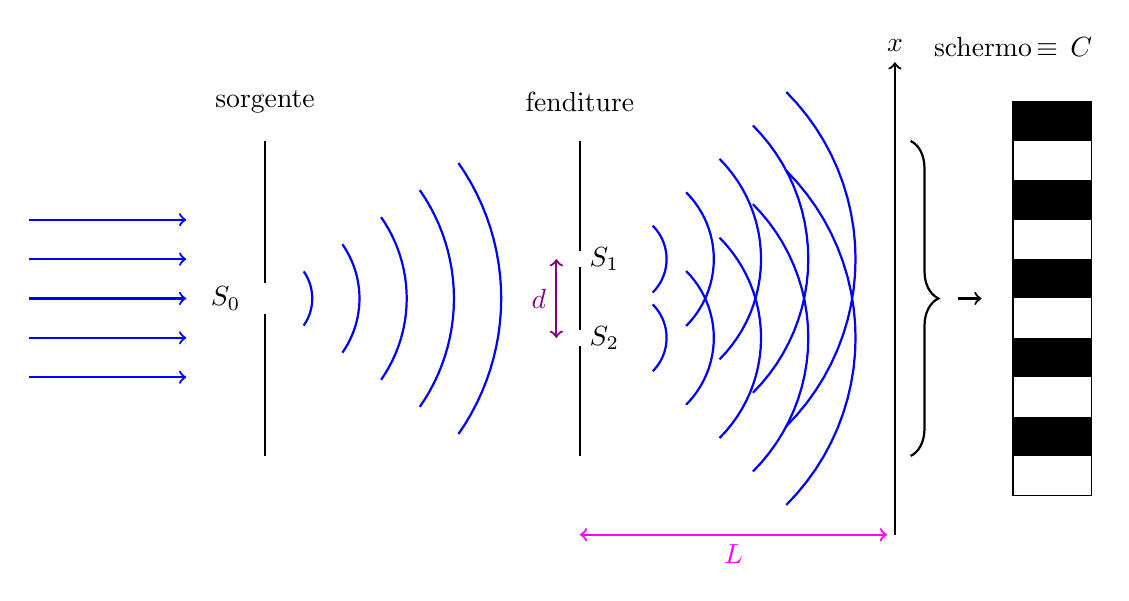
\begin{tikzpicture}
    %\draw[very thin] (-5,-5) grid (7,7);
    % Parametri
    \def\gap{1.2} % Distanza tra fenditure
    \def\L{6} % Distanza tra fenditure e schermo
    \def\screenheight{4} % Altezza dello schermo
    \def\waveRadius{2} % Raggio massimo per le onde circolari
    
    % Luce monocromatica entrnate:
    \draw[thick, blue, ->] (-9,0)--(-7,0);
    \draw[thick, blue, ->] (-9,0.5)--(-7,0.5);
    \draw[thick, blue, ->] (-9,1)--(-7,1);
    \draw[thick, blue, ->] (-9,-0.5)--(-7,-0.5);
    \draw[thick, blue, ->] (-9,-1)--(-7,-1);
    
    %Primo schermo in cui è praticata una sola fenditura
    \draw[thick] (-6,2) -- (-6,0.2);
    \draw[thick] (-6,-0.2) -- (-6,-2) node at (-6.5,0) {$S_{0}$};
    
    %Cosa esce da S0
    
    \foreach \r in {0.6, 1.2, 1.8, 2.4, 3} {
        \draw[blue,thick,domain=-35:35] plot ({\r*cos(\x)-6}, {\r*sin(\x) + 0});
        }
   
    % Schermo con doppia fenditura
    \draw[thick] (-2,-2) -- (-2,2);
    
    % Fenditure (due spazi bianchi)
    \draw[white, line width=2mm] (-2,-0.6) -- (-2,-0.4);
    \draw[white, line width=2mm] (-2,0.6) -- (-2,0.4);
    
    % Annotazione S1 e S2
    \node[right] at (-2, 0.5) {$S_1$};
    \node[right] at (-2, -0.5) {$S_2$};
    
    % Onde circolari in uscita
    \begin{scope}[shift={(0.5, 0)}]
    \foreach \r in {0.6, 1.2, 1.8, 2.4, 3} {
        \draw[blue,thick,domain=-45:45] plot ({\r*cos(\x)-2}, {\r*sin(\x)+0.5});
        \draw[blue,thick,domain=-45:45] plot ({\r*cos(\x)-2}, {\r*sin(\x)-0.5});
    }
    \end{scope}
    
    % Distanza tra fenditure (d)
    \draw[<->, thick, violet] (-2.3,0.5) -- (-2.3,-0.5) node[midway, left] at (-2.5, 0) {$d$};
    
    %Schermo finale:
    \draw[->, thick] (2,-3) -- (2,3) node[above] {$x$};
    \node at(3.5,3.2) {schermo$ \, \equiv \, C$};
    
    %label
    \node at(-6,2.5) {sorgente};
    \node at(-2,2.5) {fenditure};
    
    \draw[<->, thick, Magenta] (-2,-3) -- (1.9,-3) node[midway,below] {$L$};
    
    %frecce per le frange
    \draw[->, thick] (2.8,0) -- (3.1,0);
    %Parentesi graffa
	\draw[thick, decorate, decoration={brace, amplitude=10pt, mirror}] (2.2,-2) -- (2.2,2);    
        
    \begin{scope}[shift={(3.5,-2.5)}]
  % Disegna il rettangolo esterno: da (0,0) a (1,5)
  \draw (0,0) rectangle (1,5);
  
  % Riempie le strisce nere alternate (dall'alto verso il basso)
  \foreach \j in {0,...,4} {
    \pgfmathsetmacro{\yTop}{5 - 1*\j}
    \pgfmathsetmacro{\yBot}{5 - 1*\j - 0.5}
    \fill[black] (0,\yBot) rectangle (1,\yTop);
  }
    \end{scope}
\end{tikzpicture}
\end{center}
%%%%%%%%%%
\vspace{1em}

	Analizzando velocemente la configurazione, che abbiamo approfondito nel corso di \textit{Fisica-Generale-3}, possiamo notare che un fascio di luce monocromatica incide su uno schermo opaco sul quale sono praticate due fenditure, $S_1$ ed $S_2$, piccole e molto vicine tra loro. Nell’attraversare i fori, la luce subisce diffrazione e su una lastra fotografica, posta ad una certa distanza dallo schermo, si osservano delle frange di interferenza nella zona in cui si sovrappongono le figure di diffrazione prodotte da $S_1$ ed $S_2$.

\subsubsection{Interferenza e natura ondulatoria della luce:}
	
	 Tale esperimento fu la prova, nel lontano 1802, della natura ondulatoria della luce ed è noto ai più come \textit{esperimento di Young}. In particolare le frange di interferenza, ossia la sovrapposizione delle onde provenienti da $S_1$ e $S_2$, sono la prova incriminata che mostra le proprietà di interferenza della luce e che dunque, ne dimostra la natura ondulatoria.
	
\subsection{Interpretazione Corpuscolare della Luce}

	Come sappiamo dalle sezioni precedenti la luce è quantizzata e chiamiamo i quanti della luce, fotoni, particelle mass-less con un'energia, quantizzata, che dipende dalla formula di Einstein-Planck e che viaggiano a $c$. Ci chiediamo dunque come si interpreta il risultato in termini di queste particelle. Evidentemente dove le frange sono più luminose arrivano tanti fotoni, dove ne arrivano meno invece, sono meno luminose. Sembrerebbe quindi che i vari fotoni interagiscono tra loro in modo da dar luogo alla figura di interferenza. Ma allora cosa succede se riduciamo l'intensità della luce fino a far arrivare in media un solo fotone per volta nel percorso dalla sorgente alla lastra fotografica? Succede che dovremmo aumentare il tempo di esposizione in modo da far arrivare su di essa, in tutto, un grande numero di fotoni, e alla fine, dopo averla sviluppata, finiamo per ritrovare la stessa identica figura di interferenza. Infatti se la lastra viene sviluppata dopo una breve esposizione, su di essa osserviamo tante macchioline, disposte praticamente a caso, che sono i punti in cui sono arrivati i fotoni ed hanno prodotto la reazione chimica che impressiona la lastra; al crescere del tempo di esposizione la distribuzione delle macchioline gradatamente perde quell'apparente causalità e va invece a formare una figura di interferenza. Che conseguenza ha questo fatto?
	\\
	\\
	Significa che l'interpretazione in termini di fotoni non regge, infatti sappiamo che i fotoni non interagiscono tra di loro (poiché li "sputiamo" uno alla volta nel nostro esempio) e l'unica conclusione "semplice" è che l'interferenza dipenda dal singolo fotone (come se fosse codificata nel singolo fotone). 
	\\
	\\
	Ora però, secondo il modello corpuscolare, un fotone o passa dal foro $S_1$ o passa dal foro $S_2$. Quando passa dal foro $S_1$ è come se il foro $S_2$ fosse tappato e, viceversa, quando passa dal foro $S_2$ è come se il foro $S_1$ fosse tappato. Se l'alternativa è questa non riusciamo a spiegare il risultato sperimentale che graficamente appare come segue:

\vspace{1em}
%%%%%%%%%%%%%
\begin{center}
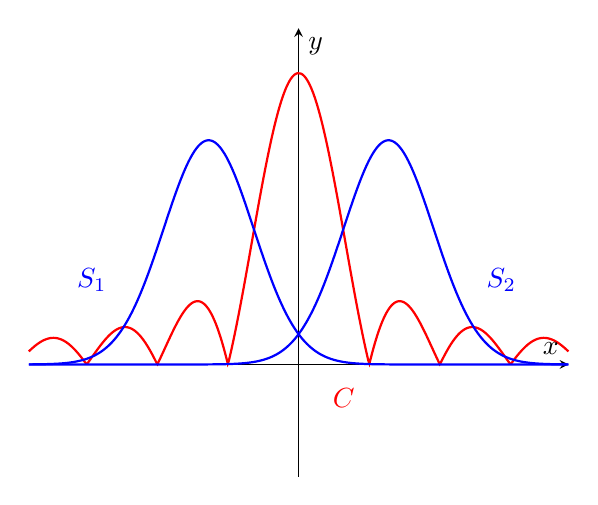
\begin{tikzpicture}

	%\draw[very thin] (0,0) grid (5,5);

	\node[red] at (4,1) {$C$};
	
	\node[blue] at (0.8,2.5) {$S_1$};
	\node[blue] at (6,2.5) {$S_2$};

  \begin{axis}[
      axis lines = center,   % gli assi al centro
      xlabel = {$x$},
      ylabel = {$y$},
      xtick=\empty,          % rimuove i tick (numeri) sull'asse x
      ytick=\empty,          % rimuove i tick (numeri) sull'asse y
      xmin=-12, xmax=12,
      ymin=-0.5, ymax=1.5,
      samples=500,
      domain=-12:12,
      clip=false,
  ]
    \addplot[red, thick] {abs(x==0 ? 1 : 1.3*sin(deg(x))/x)};
    
    \addplot[blue, thick] {exp(-((1/2)*x-2)^2 / 2)};
  
   \addplot[blue, thick] {exp(-((1/2)*x+2)^2 / 2)};
  \end{axis}
  
\end{tikzpicture}
\end{center}
%%%%%%%%%%%%%
\vspace{1em}
	
	Le figure in \textcolor{blue}{blu} come si può intuire sono le figure che si ottengono con solo $S_1$ aperto o solo $S_2$ aperto. Invece la situazione in cui $S_1$ ed $S_2$ sono entrambe aperte da origine alla \textcolor{red}{figura di interferenza finale} che chiamo \textcolor{red}{$C$}. C'è un grosso problema però con l'interpretazione corpuscolare come abbiamo accennato. La figura di interferenza infatti in questo modo non si riesce a spiegare. Immaginiamo appunto di essere un fotone che passa per $S_1$, essendo questo caso comparabile con il caso in cui solo $S_1$ è aperto mentre $S_2$ è chiuso, dovremmo poter arrivare in tutti i punti della lastra che ci indica la figura di diffrazione per $S_1$, anche in quei punti, in cui invece, la figura $C$ dice che non arrivano fotoni (frange di interferenza). Ci aspetteremmo piuttosto che $C$ fosse la somma delle intensità delle figure di diffrazione prodotte separatamente, come se la lastra dopo essere stata esposta alla luce proveniente dal solo foro $S_1$ venisse esposta alla luce uscente dal solo foro $S_2$. Il risultato invece che otteniamo non ha nulla a che fare con tutto ciò.
	
\subsection{Caso di Altre Particelle}

	Come abbiamo già detto, l'esperimento è replicabile, sotto altre configurazioni che non approfondiamo, anche con elettroni, neutroni, atomi o altre particelle. Il risultato che si ottiene è il medesimo. Quindi, ne segue che, il fenomeno non è prerogativa dei fotoni ma anche delle altre particelle. Ne segue che deve collegarsi direttamente al comportamento della singola particella in generale e non alle interazioni fra di esse.

\subsection{Stato di un Sistema}

	Introduciamo ora il concetto di \textbf{stato} di un sistema. In fisica classica, per esempio, lo stato di una particella ad un dato istante è definito dalla posizione e dalla quantità di moto della particella a quell’istante, cioè si ha un punto $\qty(x, p)$ nello spazio delle fasi. Nella nuova teoria dato che, evidentemente non è sempre possibile dire se una particella segue un percorso oppure un altro, dobbiamo essere molto prudenti con la definizione di stato. Le informazioni che definiscono lo stato di un sistema riguardano esclusivamente grandezze sotto il nostro controllo e che possiamo modificare, in generale tutto ciò che è necessario per caratterizzare completamente e riproducibilmente la situazione sperimentale. Allora, nell’esperimento di Young, lo stato $S_1$, definito dal fatto che il foro $S_2$ è tappato, è diverso dallo stato $S_2$, in cui il foro $S_1$ è tappato. Allo stesso modo, lo stato $C$, definito dal fatto che entrambi i fori sono aperti, è diverso sia da $S_1$ che da $S_2$ e non è a volte $S_1$ e ad a volte $S_2$ altrimenti non si spiega la figura, bensì è del tipo che $C$ deve "avere a che fare" sia con $S_1$ che con $S_2$. In pratica stiamo dicendo che non è corretto pensare che il fotone passi esclusivamente da $S_1$ o da $S_2$, ma deve essere considerato in uno stato quantistico (dunque che non può essere ricondotto a leggi della fisica classica) che comprende entrambe le possibilità (una sovrapposizione degli stati).

\subsection{Il Ruolo della Misura}

	Fino ad adesso abbiamo parlato in termini speculativi, però nessuno ci vieta di provare a verificare da dove sia passato, per esempio, il fotone. Cosa succede allora se realizziamo un esperimento in grado di dirci fotone per fotone da che parte è passato? Supponiamo di mettere dietro ai fori $S_1$ ed $S_2$ due fotomoltiplicatori (contatori di fotoni) $F1$ ed $F2$. Facciamo poi partire un fotone dalla sorgente, cosa ci aspettiamo?
	\\
	\\
	Chiaramente non ci aspettiamo che scattino simultaneamente altrimenti saremmo in grado di dividere a metà un fotone, ma ciò non è possibile. Ciò che si osserva è che, in media, metà delle volte scatta $F1$ e metà delle volte $F2$. Ciò significa forse che è errato pensare all’esistenza di uno stato $C$ e che forse ogni fotone è nello stato $S_1$ oppure nello stato $S_2$ e quindi $C$ è effettivamente "qualche volta A, qualche volta B". Prima di considerare buona questa conclusione, osserviamo che l’aver inserito i fotomoltiplicatori ci permette si di decidere da che parte è passato ogni fotone, ma ci preclude la possibilità di vedere le frange di interferenza: infatti i fotomoltiplicatori assorbono fotoni. Potremmo essere portati a pensare che una misura più sofisticata invece possa portarci a continuare a vedere le frange di interferenza, potremmo infatti pensare che non funzioni con i fotoni ma magari funzioni con altre particelle come i neutroni; purtroppo pensando anche ai più complessi apparati sperimentali, possiamo concludere con certezza che l'osservazione delle frange è incompatibile con la possibilità di stabilire il percorso che segue la particella.

\subsection{Conclusioni Fondamentali}

	Concludiamo questo paragrafo ricapitolando brevemente i concetti importanti introdotti:

\begin{enumerate}
	\item Le frange di interferenza si osservano anche inviando un fotone per volta: è quindi il singolo fotone ad interagire con se stesso.
	\item  Il singolo fotone non passa né da $S_1$ né da $S_2$: sussiste una terza possibilità non contemplata dalla fisica classica, cioè uno stato $C$ che, in qualche modo da stabilire, è imparentato sia con $S_1$ che con $S_2$.
	\item Una misura che mette in evidenza se il fotone è passato da $S_1$ o da $S_2$ modifica (perturba) lo stato del fotone al punto che non si vedono più le frange: o sappiamo da dove è passato ogni fotone, o vediamo le frange, non entrambe le cose.
\end{enumerate}

	L'esperimento dunque dimostra che che i fotoni non possono essere considerati esclusivamente come particelle (che passano da un solo percorso) né come onde indipendenti. La descrizione corretta è quella quantistica, in cui il fotone è in uno stato di sovrapposzione che "contiene" entrambe le possibilità.

\subsection{Cosa c'entra De Broglie?}

	"Le onde di De Broglie" vedremo, rappresentano onde di probabilità, cioè onde associate alla probabilità di trovare una particella in un dato punto dello spazio e in un certo istante di tempo. Queste onde non sono perturbazioni fisiche dirette di una sostanza o di un campo classico, ma sono legate alla descrizione quantistica dello stato di una particella. Non sono dunque né onde elastiche né onde elettromagnetiche.








